\section{Aufbau und Durchführung}
\begin{figure}[H]
  \centering
  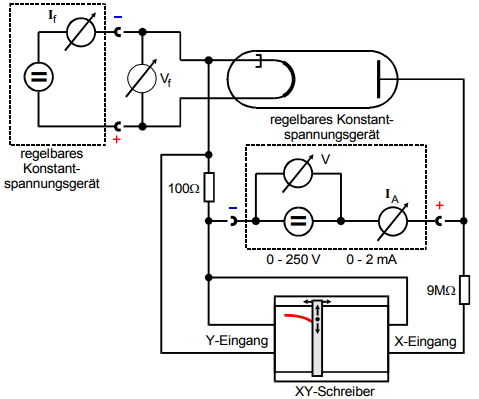
\includegraphics[width=\linewidth-100pt,height=\textheight-100pt,keepaspectratio]{Text/Bilder/Schaltung1.png}
  \caption{Darstellung einer möglichen Schaltung zur Aufnahme von Kennlinien mit $V\ge0$ \cite[101]{sample}}
  \label{fig:Schaltung1}
\end{figure}
Zur Messung einer Kennlinienschar wird  zunächst die in Abbildung \ref{fig:Schaltung1} zu sehende Schaltung aufgebaut. Daraufhin wird ein Heizstrom zwischen $2.0$ und $\SI{2.5}{V}$ eingestellt und die dazugehörige Spannung gemessen.
Anschließend wird die Saugspannung zwischen $0$ und $\SI{110}{V}$ in regelmäßigen Abständen variiert. Diese und die dazugehörende Stromstärke werden in $10$ bis $20$ Wertepaaren notiert.
Der Vorgang wird für 4 weitere Heizspannungen wiederholt.
\begin{figure}[H]
	\centering
	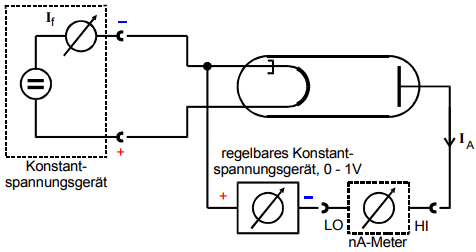
\includegraphics[width=\linewidth-100pt,height=\textheight-100pt,keepaspectratio]{Text/Bilder/Schaltung2.png}
	\caption{Darstellung einer möglichen Schaltung zur Aufnahme von Kennlinien mit $V\le0$ \cite[102]{sample}.}
	\label{fig:Schaltung2}
\end{figure}
Im zweiten Teil der Messung  wird zum Erstellen einer Kennlinie im Anlaufstromgebiet die
Schaltung aus Abbildung \ref{fig:Schaltung2} aufgebaut.
Daraufhin wird die Gegenspannung von $0$ bis $-\SI{1}{V}$ variiert und zusammen mit der zugehörigen Anlaufstromstärke notiert.
